% === Impostazione del documento ==========================
\documentclass[11pt, openany]{extbook}

\usepackage[english,italian]{babel}
\usepackage{setspace}
\onehalfspace

%=== Allinameto testo a sinistra =========================
\setlength{\parindent}{0pt}


% === Regolazione dei margini =============================
\addtolength{\oddsidemargin}{30pt}
\addtolength{\evensidemargin}{-30pt}
\usepackage{fancyhdr}
\usepackage{multirow}
\usepackage{multicol} 
\usepackage[section]{placeins}

%=== CODICE  =========================
\usepackage{xcolor}
\definecolor{commentgreen}{RGB}{2,112,10}
\definecolor{eminence}{RGB}{108,48,130}
\definecolor{weborange}{RGB}{255,165,0}
\definecolor{frenchplum}{RGB}{129,20,83}
\definecolor{dkgreen}{rgb}{0,0.6,0}
\definecolor{gray}{rgb}{0.5,0.5,0.5}
\definecolor{mauve}{rgb}{0.58,0,0.82}

\usepackage{listings}
\lstset {
    language= C,
    frame=tb,
    tabsize=4,
    showstringspaces=false,
    numbers=left,
    %upquote=true,
    commentstyle=\color{commentgreen},
    keywordstyle=\color{eminence},
    stringstyle=\color{red},
    basicstyle=\small\ttfamily, % basic font setting
    emph={int,char,double,float,unsigned,void,bool},
    emphstyle={\color{blue}}, % keyword highlighting
    classoffset=1, % starting new class
    otherkeywords={>,<,.,;,-,!,=,~},
    morekeywords={>,<,.,;,-,!,=,~},
    keywordstyle=\color{weborange},
    classoffset=0
}

\lstset{
  language=R,                     % the language of the code
  basicstyle=\footnotesize,       % the size of the fonts that are used for the code
  numbers=left,                   % where to put the line-numbers
  numberstyle=\tiny\color{gray},  % the style that is used for the line-numbers
  stepnumber=1,                   % the step between two line-numbers. If it's 1, each line
                                  % will be numbered
  numbersep=5pt,                  % how far the line-numbers are from the code
  backgroundcolor=\color{white},  % choose the background color. You must add \usepackage{color}
  showspaces=false,               % show spaces adding particular underscores
  showstringspaces=false,         % underline spaces within strings
  showtabs=false,                 % show tabs within strings adding particular underscores
  frame=tb,                   % adds a frame around the code
  rulecolor=\color{black},        % if not set, the frame-color may be changed on line-breaks within not-black text (e.g. commens (green here))
  tabsize=2,                      % sets default tabsize to 2 spaces
  captionpos=b,                   % sets the caption-position to bottom
  breaklines=true,                % sets automatic line breaking
  breakatwhitespace=false,        % sets if automatic breaks should only happen at whitespace
  title=\lstname,                 % show the filename of files included with \lstinputlisting;
                                  % also try caption instead of title
  keywordstyle=\color{blue},      % keyword style
  commentstyle=\color{dkgreen},   % comment style
  stringstyle=\color{mauve},      % string literal style
  escapeinside={\%*}{*)},         % if you want to add a comment within your code
  morekeywords={*,...}            % if you want to add more keywords to the set
} 


% === Integrazione delle figure ===========================
\usepackage{graphicx}
\usepackage{wrapfig}
\graphicspath{{./imgs/}}
\renewcommand{\figurename}{Fig.}
\usepackage{subfigure}
\usepackage[section]{placeins}
\usepackage[nottoc]{tocbibind}

% === Link Url ============================================
% riferimenti cliccabili nel pdf
\usepackage[pdftex]{hyperref}

% Impostazione dei link nel pdf
\hypersetup{%
    colorlinks=true,
    citecolor=green,
    linkcolor=darkgray,
    urlcolor=red,
}   

% === Per le tabelle ======================================
\usepackage{tabularx}
\usepackage{multirow}

% === Per la bibliografia multicolonna ====================
\usepackage{etoolbox}
%\usepackage[backend=biber, sorting=none]{biblatex} \addbibresource{bibliografia-tesi.bib}

%\patchcmd{\thebibliography}{\list}{\begin{multicols}{2}\smaller\list}{}{}
%\appto{\endthebibliography}{\end{multicols}}
% === Per il testo di prova =================================
\usepackage{lipsum}

%%%%%%%%%%%%%%%%%%%%%%%%%%%%%%%%%%%%%%%%%%%%%%%%%%%%%%%%%%%
% TESTO DELLA TESI
%%%%%%%%%%%%%%%%%%%%%%%%%%%%%%%%%%%%%%%%%%%%%%%%%%%%%%%%%%%

\begin{document}
\frontmatter

	% === Frontespizio ====================================
	\pagestyle{empty}
	%%%%%%%%%%%%%%%%%%%%%%%%%%%%%%%%%%%%%%%%%%%%%%%%%%%%%%%%%%%
% Frontespizio
%%%%%%%%%%%%%%%%%%%%%%%%%%%%%%%%%%%%%%%%%%%%%%%%%%%%%%%%%%%

\begin{titlepage}
 \begin{center}
     
\includegraphics[width=3.5cm]{Learning/09_ReadME_Documentazione/0_frontespizio/imgs/unimol/unimol_color.png}\\
     \vspace{2em}
     {\Large \textsc{Università  degli studi del Molise}}\\
     \vspace{1em}
     %{\Large \textsc{Corso di Laurea Magistrale in}}\\
     \vspace{1em}
      %{\Large \textsc{Sicurezza dei Sistemi Software }}\\
     \vspace{2em}
     \vspace{4em}
     {\LARGE\textbf{
     ReadMe\\ Documentazione \& Convenzioni\\
       \vspace{1em}
     }}
\begin{center}
     \LARGE{Project Management \& Ingegneria del software} 
\end{center}
 \end{center}

\begin{center}
  \vspace{\fill} %TESTO A FINE PAGINA
{\normalsize Anno Accademico 2021/2022}
\end{center}
\end{titlepage}

\clearpage{\pagestyle{empty}\cleardoublepage}

    
	

	
	% === Indice ==========================================
    \tableofcontents
    \listoffigures



	% === Capitoli Tesi ===================================
	\mainmatter 
	\pagestyle{plain}
	\newpage
	\chapter{Daily Scrum Documentation}
\label{chap:dailyscrum}
\section{Cos'è il Daily Scrum?}
Lo scopo di questo documento è tenere traccia del lavoro giornaliero svolto da ogni membro del team. Nel nostro caso ogni team (Frontend e Backend) avrà il suo documento del Daily Scrum dedicato:
\begin{itemize}
    \item FE - Daily Scrum \href{https://studentiunimol-my.sharepoint.com/:x:/r/personal/a_daguanno1_studenti_unimol_it/_layouts/15/Doc.aspx?sourcedoc=\%7BC6890990-B5A6-4D9F-9306-993B687826C0\%7D&file=FE\%20-\%20Daily\%20Scrum.xlsx&action=default&mobileredirect=true}{[Drive Frontend]}
    \item BE - Daily Scrum \href{https://studentiunimol-my.sharepoint.com/:x:/r/personal/a_daguanno1_studenti_unimol_it/_layouts/15/Doc.aspx?sourcedoc=\%7BDC32CDAD-D25E-4F03-9490-1BA4A0895567\%7D&file=BE\%20-\%20Daily\%20Scrum.xlsx&action=default&mobileredirect=true}{[Drive Backend]}
\end{itemize}

Ogni Sprint ha la durata di 2 settimane di conseguenza il documento ha due tabelle da compilare nelle due settimane (week) ed i differenti fogli rappresentano i vari sprint che ci saranno durante il progetto.\\
Il primo sprint (\textbf{Sprint n.1}) va dal 30/03 al 12/04. E la prima settimana dal 30/03 al 05/04 \small{[fig:\ref{fig:week}]}

\begin{figure}[ht]
    \centering
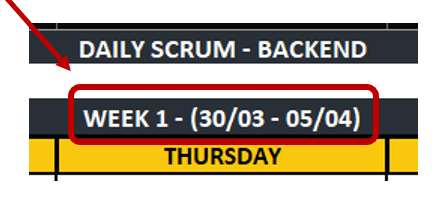
\includegraphics[width=0.7\textwidth]{Learning/09_ReadME_Documentazione/1_DailyScrumDoc/img_DSD/Immagine 2022-04-01 222626.png}
    \caption{suddivisione settimanale della tabella}
    \label{fig:week}
    \end{figure}
\FloatBarrier
\begin{figure}[ht]
    \centering
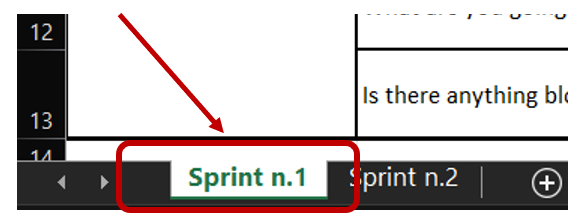
\includegraphics[width=0.7\textwidth]{Learning/09_ReadME_Documentazione/1_DailyScrumDoc/img_DSD/Immagine 2022-04-01 223141.png}
    \caption{fogli per la suddivisione degli Sprint}
    \label{fig:scrum}
    \end{figure}
\FloatBarrier

% ==============================================================================================================================
\newpage
\section{Come compilare il documento}
Ogni membro del team deve \underline{quotidianamente} rispondere alle 3 domande che compongono questo documento: 
\begin{enumerate}
    \item \textbf{What did you do yesterday?} - Descrivere ciò che è stato completato il giorno precedente.  
    \item \textbf{What are you going to do today?} - I progressi che si hanno in programma di fare.
    \item \textbf{Is there anything blocking you?} - Riportare i problemi che rallentano il workflow delle issue. 
\end{enumerate}

\subsection{Accedere al documento}
Ogni Team (FE e BE) ha una propria cartella dedicata sul Drive con tutti i file della documentazione relativi. I link sono presenti nel relativo canale \textbf{daily-scrum} del server Discord.\\
Il file si compila direttamente dall'editor online, in questo modo lavoriamo tutti sullo stesso file che sarà sempre aggiornato.\\
Chi vuole può creare una copia di backup che però non deve essere caricata nella cartella condivisa. 
	\chapter{Convenzioni Git}
\label{chap:convenzioni}


\section{Best practice per il branching}
    \begin{itemize}
        \item Lavorare sempre su branch propri
        \item Staccare i branch da staging (versione stabile della repository)
        \item Nominare il branch con la specifica della funzionalità da implementare (Es. branch: update-users-api)
        \item Aggiornare il proprio branch prima di ogni merge request (attraverso il pull da staging)
        \item Assegnare la merge request al scrum master di riferimento (Eg. Backend: Assignee -> Alessandro)
    \end{itemize}

\section{Best practice per le commit}
    \subsection{Creazione delle commit}
        \begin{itemize}
            \item Aggiungere nella commit solo i cambiamenti relativi ad una singola funzionalità. Evitare quindi di creare delle commit di grosse dimensioni, contenenti modifiche di diverso genere. 
            \item Testare accuratamente le funzionalità interessate prima di ogni commit.
            \item Aggiornare il file .gitignore in caso di aggiunta file spuri.
        \end{itemize}
    
    \subsection{Scrittura delle commit}
        \begin{itemize}
            \item Specificare il tipo di operazione effettuata
            \item Specificare l’identificativo della issue risolta
            \item Specificare, con un breve messaggio [max 50 caratteri] in lingua inglese, l’operazione che è stata effettuata nella commit 
        
        \end{itemize}

\subsubsection{Template}

\begin{large}
\centering{ git commit -m “\{Method\} \#\{id-issue\} – \{Commit message\}”}
\end{large}

\subsubsection{Esempi}
\textbf{Implementazione di una nuova funzionalità:}
\begin{center}
    git commit -m “Implementation \#23 – Add get all users API”
\end{center}
\medskip \medskip
%=================================================================================
\textbf{Aggiornamento di una funzionalità implementata in precedenza: }
\begin{center}
    git commit -m “Update \#11 – Remove unused fields to UserDto class”
\end{center}
\medskip \medskip
%=================================================================================
\textbf{Risoluzione di un bug o di una issue: }
\begin{center}
    git commit -m “Fix  \#103 – Fix delete user API issue”
\end{center}
\medskip \medskip
%=================================================================================
Qualora dovesse risultare necessaria una commit non associata a nessuna Issue, procedere semplicemente con il messaggio della commit.\\
\textbf{Esempi: }
\begin{center}
    \begin{itemize}
        \item git commit -m “Code refactoring” 
        \item git commit -m “Remove unused DTOs”
    \end{itemize}
\end{center}

	


	% === Bibliografia ====================================
	\newpage
	\bibliographystyle{IEEEtran}
	\bibliography{bibliografia-tesi.bib}

\end{document}

%%%%%%%%%%%%%%%%%%%%%%%%%%%%%%%%%%%%%%%%%%%%%%%%%%%%%%%%%%%
